\subsubsection{UC\theuccount-GP - Uscita dell'utente dal sistema}
%		\begin{figure}[H]
%			\centering
%				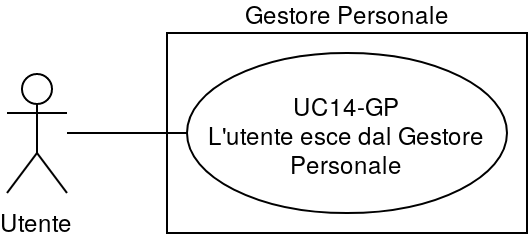
\includegraphics[width=0.7\columnwidth]{img/casi_d'uso/UC14.png}\\
%			\caption{UC\theuccount-GP - Uscita dell'utente dal sistema}
%		\end{figure}
	\begin{itemize}
		\item \textbf{Codice}: UC\theuccount-GP.
		\item \textbf{Titolo}: uscita dell'utente dal sistema.
		\item \textbf{Attori primari}: utente.
		\item \textbf{Descrizione}: l'utente esce dal sistema ed ha la possibilità di rientrarci come	un diverso utente o come lo stesso di prima.
		\item \textbf{Precondizione}: l'utente è all'interno del sistema.
		\item \textbf{Postcondizione}: l'utente è ora un utente non acceduto e si trova a poter accedere nuovamente nel sistema.
		\item \textbf{Scenario principale}:
		\begin{enumerate}
			\item L'utente riconosciuto dal sistema effettua l'uscita dallo stesso
		\end{enumerate}
	\end{itemize}